\documentclass[12pt, a4paper]{article}
\usepackage[utf8]{inputenc}
\usepackage{amsmath, amssymb} 
\usepackage{graphicx} 
\usepackage{booktabs}
\usepackage{geometry}
\usepackage{hyperref}
\usepackage{caption}
\usepackage{subcaption}
\usepackage{cite}
\usepackage{tikz}
\usepackage{threeparttable}  
\usepackage{booktabs}      
\usepackage[table]{xcolor}   
\usepackage{float}           
\usetikzlibrary{arrows.meta, patterns}
\geometry{
    top=1in,
    bottom=1in,
    left=1in,
    right=1in
}
\title{Irreversible Loss Reduction in Mathematically Continuous Asymmetric Duct Contractions}  
\date{March 12, 2026}
\begin{document}

\maketitle

\begin{abstract}
	This study presents a comparative numerical investigation of steady laminar flow through an asymmetric duct contraction, quantifying how geometric continuity influences irreversible pressure loss and boundary-layer development. Three contraction profiles are examined: a sudden step, a cosine-bell transition, and a cubic Bézier transition. The incompressible Navier--Stokes equations are solved in OpenFOAM at $Re=232$, with numerical reliability established through a three-level Grid Convergence Index (GCI) analysis on meshes up to $2.36 \times 10^6$ cells ($h=0.5$ mm). The fine-grid GCI remains below $2\%$, confirming asymptotic grid independence. While the cubic Bézier profile achieved the lowest inlet kinematic pressure ($4.88\ \mathrm{m^2/s^2}$), streamline visualization indicates a localized viscous accumulation at its entry junction due to a higher initial curvature change. In contrast, the cosine-bell profile ($5.19$~m$^2$/s$^2$) exhibits a more gradual entry 
	and retains a $2.97\%$ higher kinetic energy flux at the outlet plane 
	($1.04 \times 10^{-3}$ vs $1.01 \times 10^{-3}$~m$^4$/s$^2$), confirming 
	thermodynamic superiority despite its higher inlet kinematic pressure requirement. 
	This demonstrates that while the cubic B\'{e}zier profile minimises inlet 
	kinematic pressure, the cosine-bell profile achieves superior overall energy 
    conservation across the contraction. Bernoulli-based validation shows an outlet-velocity deviation of only $1.80\%$, consistent with viscous boundary-layer growth. These results demonstrate that while $C^1$ continuity suppresses the macroscopic vena contracta, hydraulic efficiency is governed by the spatial distribution of curvature rather than endpoint smoothness alone.
	\end{abstract}


\vspace{0.5cm}
\noindent \textbf{Keywords:}  Steady Incompressible Navier–Stokes, Computational Fluid Dynamics (CFD), Irreversible Pressure Loss, Laminar Internal Flow, Vena Contracta, Recirculation, Bernoulli Equation, Darcy-Weisbach Equation, Grid Convergence Index (GCI).

\newpage

\section*{Nomenclature}

\subsection*{Roman Symbols}
\begin{tabular}{lll}
	$h$             & Grid spacing                               & [mm] \\
	$h_{max}$       & Maximum edge length in mesh                         & [mm] \\
	$L_r$           & Reattachment length                                 & [mm] \\
	$Re$            & Reynolds number                                     & [-] \\
	$x$             & Axial position              & [mm] \\
\end{tabular}

\subsection*{Greek Symbols}
\begin{tabular}{lll}
	$\delta^*$      & Displacement thickness                               & [mm] \\
    $\Phi$        & Kinematic pressure & [m$^2$/s$^2$] \\
	$\rho$          & Fluid density                                                         & [kg/m$^3$] \\
	$\tau_w$        & Wall shear stress             & [Pa] \\
	$\sigma$        & Contraction Ratio             & [-]  \\
	$\psi$        & Energy Flux     & [m$^4$/s$^2$] \\
	
\end{tabular}

\subsection*{Abbreviations}
\begin{tabular}{ll}
	AMR             & Adaptive Mesh Refinement                             \\
	CFD             & Computational Fluid Dynamics                         \\
	GCI             & Grid Convergence Index                               \\
	PIV             & Particle Image Velocimetry                           \\
\end{tabular}

\subsection*{Mesh Quality Metrics}
\begin{tabular}{ll}
	Max. Skewness       & Measure of cell equiangularity                  \\
	Max. Non-Orth.      & Maximum angle between face normal and cell centroids \\
	Max. Aspect Ratio   & Ratio of maximum to minimum cell dimensions      \\
\end{tabular}
\newpage
\section{Introduction}
Flows completely bounded by solid surfaces are classified as \textit{internal flows.} Thus internal flows include flows through pipes, ducts, nozzles, diffusers, sudden contractions and expansions, valves, and fittings \cite{fox2020}.
These flows may be laminar or turbulent which can be categorized by a dimensionless quantity \textit{Reynolds Number} Re named after Reynolds (1883) and mathematically defined by $Re = \frac{v L}{\nu}$, where \textit{v} and \textit{L} represent characteristic average flow velocity and characteristic length. Laminar flow typically occurs when $Re < 2300$. 

To characterize pressure losses, the relationship between the pressure head loss $h_L$ and the mean flow velocity $v$ can be characterized by a power law governed by the exponent $\alpha$:

\begin{equation}
	h_L \propto v^{\alpha}
\end{equation}

where the value of $\alpha$ depends on the flow regime as follows:

\begin{equation}
	\alpha = 
	\begin{cases} 
		1 & \text{for Laminar Flow } (Re < 2300) \\
		1.75 \text{ to } 2.0 & \text{for Turbulent Flow } (Re > 4000)
	\end{cases}
\end{equation}

In the laminar regime, the pressure drop is dominated by viscous forces, resulting in a linear dependency ($\alpha = 1$). As the flow transitions to turbulence, the dependency becomes non-linear due to the dominance of inertial effects and momentum exchange, with $\alpha$ typically approaching $1.75$ for smooth pipes (Blasius regime) and $2.0$ for fully rough conditions.\cite{white2016}


Internal flow through duct contractions is a fundamental phenomenon in mechanical systems, appearing in applications ranging from industrial piping networks to high-precision microfluidic cooling channels. The primary challenge in these systems is the management of energy efficiency, which is often dictated by the geometric transitions within the flow path. In conventional "sudden" contractions, the fluid streamlines are unable to negotiate the abrupt 90$^\circ$ geometric discontinuity, leading to immediate boundary layer separation at the leading edge. This separation triggers the formation of a vena contracta, where the effective flow area is significantly reduced, resulting in localized high-velocity gradients and intense viscous dissipation.

These localized physical phenomena generate substantial irreversible kinematic pressure losses ($p/\rho$) in laminar regimes. The primary driver of this inefficiency is the creation of large recirculation zones immediately downstream of the contraction throat. To mitigate these losses, geometric optimization strategies focus on providing a smooth transition profile that guides streamlines along the wall boundaries, thereby maintaining flow attachment and suppressing the formation of recirculation eddies. While various linear and curved profiles are utilized in engineering practice, the implementation of a mathematically disciplined, parametric transition is essential for ensuring tangential smoothness ($C^1$ continuity) \cite{piegl1996nurbs} at the junction points. $C^1$ continuity ensures that both position and slope are continuous across geometric junctions.

\subsection{Mathematical Definition of $C^1$ Continuity}

For a geometric transition between two parametric curves, $\mathbf{r}_1(s)$ and $\mathbf{r}_2(t)$, to achieve $C^1$ continuity at a common junction point $P$, two conditions must be satisfied:

\begin{enumerate}
	\item \textbf{$C^0$ Continuity (Position)}: The curves must meet at the same spatial coordinates:
	\begin{equation}
		\mathbf{r}_1(s_{max}) = \mathbf{r}_2(t_{min}) = P
	\end{equation}
	
	\item \textbf{$C^1$ Continuity (Tangent Vector)}: The first derivatives (tangent vectors) must be equal in both magnitude and direction at the junction:
	\begin{equation}
		\frac{d\mathbf{r}_1}{ds}\Big|_{s_{max}} = \frac{d\mathbf{r}_2}{dt}\Big|_{t_{min}}
	\end{equation}
\end{enumerate}

\begin{figure}[htbp]
	\centering
	\includegraphics[width=0.9\textwidth]{C1_continuity}
	\caption{Comparison between \textit{G1} and \textit{C1} continuity connections. The \textit{C1} continuity shown on the right ensures first-derivative smoothness, which is critical for maintaining attached streamlines in duct contractions.}
	\label{fig:c1_vis}
\end{figure}

In the specific case of the cosine-bell profile \ref{fig:cosine_asym}, $C^1$ continuity ensures that the slope of the wall transition perfectly matches the horizontal duct walls at the inlet and outlet. This mathematical smoothness substantially reduces the geometric singularity that otherwise triggers the formation of a vena contracta and its associated energy dissipation.  
The governing physics of the duct flow are described by the steady incompressible Navier-Stokes partial differential equations (\textit{PDEs}), where the viscous term $\nu \nabla^2 \mathbf{u}$ necessitates a high degree of geometric smoothness for numerical stability and physical accuracy. In a conventional sudden contraction, the geometry exhibits only $C^0$ continuity (positional only), creating a singularity in the boundary slope at the corner.

Mathematically, we define the required $C^1$ continuity at a junction point $x_c$ using the limit definition of the derivative. For a wall profile function $f(x)$ to be $C^1$ continuous, the left-hand and right-hand limits of the first derivative must be equal:
\begin{equation}
	\lim_{h \to 0^-} \frac{f(x_c + h) - f(x_c)}{h} = \lim_{h \to 0^+} \frac{f(x_c + h) - f(x_c)}{h} = f'(x_c)
\end{equation}
In a sudden $90^\circ$ contraction, this equality fails because the slope jumps from $0$ to undefined (infinite), leading to an immediate separation of the boundary layer as the fluid streamlines cannot negotiate the discontinuity. By implementing a cosine-bell profile, we ensure that the first derivative is continuous across all junction points. This maintains a finite and continuous pressure gradient $\nabla p$ in the momentum partial differential equation (\textit{PDE}), which substantially suppresses the formation of the vena contracta and the associated energy dissipation identified in empirical benchmarks.

\section{Governing Equations}

Following the formulation presented by Chorin and Marsden\footnotemark[1], the motion of an incompressible, viscous Newtonian fluid is governed by the conservation of mass and the balance of momentum \cite{chorin1993}. \footnotetext[1]{Based on a one-term course in fluid mechanics originally taught in the \textit{Department of Mathematics} of the \textit{University of California, Berkeley}, during the spring of 1978.}



\subsection{Dimensional Formulation}
Let $\mathbf{u}(\mathbf{x}, t)$ be the velocity vector field and $p(\mathbf{x}, t)$ be the scalar pressure field. For a fluid with constant density $\rho$ and dynamic viscosity $\mu$, the Navier-Stokes equations (NSE) in a domain $D \subset \mathbb{R}^3$ are expressed as:

\begin{equation}
	\nabla \cdot \mathbf{u} = 0
\end{equation}
\begin{equation}
	\rho \left( \frac{\partial \mathbf{u}}{\partial t} + (\mathbf{u} \cdot \nabla)\mathbf{u} \right) = -\nabla p + \mu \nabla^2 \mathbf{u}
\end{equation}
where the non-linear term $(\mathbf{u} \cdot \nabla)\mathbf{u}$ represents the convective acceleration and $\nabla^2 \mathbf{u}$ represents the diffusion of momentum due to viscosity.

Mathematically, the \textit{material} or \textit{substantial} derivative is expressed as:
\begin{equation}
\frac{D}{Dt} = \frac{\partial}{\partial t} + (\mathbf{u} \cdot \nabla)
\end{equation}
Using this operator, the incompressible Navier-Stokes equation in their dimensional form is:
\begin{equation}
\rho \frac{D\mathbf{u}}{Dt} = -\nabla p + \mu \nabla^2 \mathbf{u}
\end{equation}

where $\mathbf{u}$ is the velocity vector, $p$ is the static pressure, $\rho$ is the constant density, and $\mu$ is the dynamic viscosity.


\subsection{Non-Dimensionalization}
To analyze the flow independently of specific units and to identify the dominant physical regimes, we introduce the following characteristic scales:
\begin{itemize}
	\item $L$: Characteristic length (e.g., the hydraulic diameter of the duct).
	\item $U$: Characteristic velocity (e.g., the mean inlet velocity).
	\item $L/U$: Convective time scale.
	\item $\rho U^2$: Dynamic pressure scale.
\end{itemize}

We define the dimensionless variables (denoted by asterisks) as:
\begin{equation}
	\mathbf{x}^* = \frac{\mathbf{x}}{L}, \quad \mathbf{u}^* = \frac{\mathbf{u}}{U}, \quad t^* = \frac{t}{L/U}, \quad p^* = \frac{p}{\rho U^2}
\end{equation}

Substituting these into the momentum equation (Eq. 7) and applying the chain rule ($\nabla = \frac{1}{L} \nabla^*$ and $\frac{\partial}{\partial t} = \frac{U}{L} \frac{\partial}{\partial t^*}$), we obtain:
\begin{equation}
	\rho \left( \frac{U^2}{L} \frac{\partial \mathbf{u}^*}{\partial t^*} + \frac{U^2}{L} (\mathbf{u}^* \cdot \nabla^*)\mathbf{u}^* \right) = -\frac{\rho U^2}{L} \nabla^* p^* + \frac{\mu U}{L^2} \nabla^{*2} \mathbf{u}^*
\end{equation}

Dividing the entire equation by the inertial scaling factor $\frac{\rho U^2}{L}$ yields the non-dimensional Navier-Stokes equation:
\begin{equation}
	\frac{\partial \mathbf{u}^*}{\partial t^*} + (\mathbf{u}^* \cdot \nabla^*)\mathbf{u}^* = -\nabla^* p^* + \frac{\mu}{\rho U L} \nabla^{*2} \mathbf{u}^*
\end{equation}

\subsection{The Dimensionless Governing Parameter}
The coefficient of the viscous term appearing in Eq. 12 is the reciprocal of the Reynolds number ($Re$), which characterizes the ratio of inertial forces to viscous forces:
\begin{equation}
	Re = \frac{\rho U L}{\mu} = \frac{U L}{\nu}
\end{equation}

Thus, for the steady-state laminar flow investigated in this study, the governing equations reduce to:
\begin{equation}
	\nabla^* \cdot \mathbf{u}^* = 0
\end{equation}
\begin{equation}
	(\mathbf{u}^* \cdot \nabla^*)\mathbf{u}^* = -\nabla^* p^* + \frac{1}{Re} \nabla^{*2} \mathbf{u}^*
\end{equation}

At the studied $Re \approx 232$, the $1/Re$ term provides sufficient momentum diffusion to suppress the transition to turbulence. However, in the sudden contraction, inertia still overcomes viscous forces at the sharp corner, leading to a steady laminar recirculation zone. The $C^1$ continuous cosine-bell profile mitigates this by smoothing the pressure gradient $\nabla^* p^*$, allowing the viscous forces to maintain attached streamlines.

The governing physics are described by the conservation of mass (continuity equation) and the conservation of momentum (Navier-Stokes equations).

\subsection{Mass Conservation}
As mentioned earlier, for an incompressible fluid, the continuity equation requires that the velocity field $\mathbf{u}$ remains divergence-free:
\begin{equation}
	\nabla \cdot \mathbf{u} = 0
\end{equation}

\subsection{Momentum Conservation}
For the present study the flow is assumed steady, incompressible, and laminar, therefore the temporal acceleration term $\frac{\partial \mathbf{u}}{\partial t}$ vanishes and the governing momentum equation reduces to:

\begin{equation}
	\rho (\mathbf{u} \cdot \nabla)\mathbf{u} = -\nabla p + \mu \nabla^2 \mathbf{u}
\end{equation}
In the context of the kinematic pressure ($p' = p/\rho$) and the kinematic viscosity ($\nu = \mu/\rho$) typically utilized by incompressible solvers, the equation (17) is expressed as:
\begin{equation}
	(\mathbf{u} \cdot \nabla)\mathbf{u} = -\nabla p' + \nu \nabla^2 \mathbf{u}
\end{equation}
where $\mathbf{u}$ is the velocity vector, $p'$ is the kinematic pressure, and $\nu$ is the kinematic viscosity of the fluid.

\section{Geometrical Modelling}

The computational domain represents a two-dimensional internal duct. This section defines the baseline sudden contraction geometry, which serves as the reference for evaluating the performance of the optimized cosine-bell profile. Geometry was implemented using FreeCAD \cite{freecad}.
\subsection{Sudden Contraction Baseline}

\noindent
\begin{minipage}{0.48\textwidth}
	The sudden contraction is the reference geometry for this study. In this configuration, the lower wall remains a straight, continuous boundary, while the upper wall undergoes a step-change in height at $x = L_{inlet}$. The upper wall profile $y(x)$ is defined as:
	
	\begin{equation}
		y(x) = 
		\begin{cases} 
			H_{in} & \text{for } 0 \leq x < L_{inlet} \\
			H_{out} & \text{for } L_{inlet} \leq x \leq L_{total}
		\end{cases}
	\end{equation}
	
	where $H_{in} = 40\,\text{mm}$, $H_{out} = 18\,\text{mm}$, $L_{inlet} = 100\,\text{mm}$ and $L_{outlet} = 50\,\text{mm}$. This $C^0$ discontinuity at the contraction plane ($x = L_{inlet}$) creates a geometric singularity. The resulting infinite pressure gradient at the sharp corner triggers flow separation and the formation of a \textit{vena contracta}, leading to the significant irreversible losses identified in the baseline simulation.
\end{minipage}
\hfill
\begin{minipage}{0.48\textwidth}
	\centering
	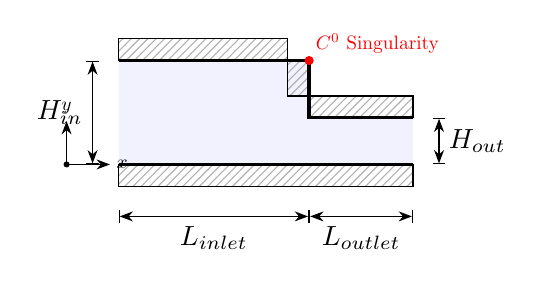
\begin{tikzpicture}[scale=1.1, >=Stealth]
		% --- Parameters ---
		\def\Li{2.2}    % Inlet Length
		\def\Lo{1.2}    % Outlet Length
		\def\Hi{1.2}    % 40mm scaled
		\def\Ho{0.54}   % 18mm scaled
		\def\wall{0.25} % Wall thickness
		
		% --- Fluid Domain ---
		\fill[blue!5] (0, 0) -- (\Li+\Lo, 0) -- (\Li+\Lo, \Ho) -- (\Li, \Ho) -- (\Li, \Hi) -- (0, \Hi) -- cycle;
		
		% --- Wall Hatching (Upper Only Contraction) ---
		% Top Wall
		\draw[pattern=north east lines, pattern color=gray!60] 
		(0, \Hi) -- (\Li, \Hi) -- (\Li, \Ho) -- (\Li+\Lo, \Ho) -- 
		(\Li+\Lo, \Ho+\wall) -- (\Li-\wall, \Ho+\wall) -- (\Li-\wall, \Hi+\wall) -- (0, \Hi+\wall) -- cycle;
		% Bottom Wall (Straight)
		\draw[pattern=north east lines, pattern color=gray!60] 
		(0, 0) -- (\Li+\Lo, 0) -- (\Li+\Lo, -\wall) -- (0, -\wall) -- cycle;
		
		% --- Boundaries ---
		\draw[very thick] (0, \Hi) -- (\Li, \Hi) -- (\Li, \Ho) -- (\Li+\Lo, \Ho); % Upper
		\draw[very thick] (0, 0) -- (\Li+\Lo, 0); % Lower (Straight)
		
		% --- Vertical Dimensions ---
		\draw[|<->|] (-0.3, 0) -- (-0.3, \Hi) node[midway, left] {$H_{in}$};
		\draw[|<->|] (\Li+\Lo+0.3, 0) -- (\Li+\Lo+0.3, \Ho) node[midway, right] {$H_{out}$};
		
		% --- Horizontal Dimensions ---
		\draw[|<->|] (0, -0.6) -- (\Li, -0.6) node[midway, below] {$L_{inlet}$};
		\draw[|<->|] (\Li, -0.6) -- (\Li+\Lo, -0.6) node[midway, below] {$L_{outlet}$};
		
		% --- Coordinate System ---
		\draw[->] (-0.6, 0) -- (-0.1, 0) node[right, scale=0.7] {$x$};
		\draw[->] (-0.6, 0) -- (-0.6, 0.5) node[above, scale=0.7] {$y$};
		\fill (-0.6, 0) circle (1pt);
		
		% --- Singularity Point ---
		\fill[red] (\Li, \Hi) circle (1.5pt);
		\node[red, anchor=south west, scale=0.7] at (\Li, \Hi) {$C^0$ Singularity};
	\end{tikzpicture}
	\captionof{figure}{Baseline geometry with an asymmetric sudden contraction and straight lower wall.}
	\label{fig:sudden_asym}
\end{minipage}

\subsection{Mathematical Singularity and Flow Separation}
This geometry exhibits only $C^0$ continuity. At the contraction plane $x = L_{inlet}$, the slope $y'(x)$ is discontinuous. When coupled with the steady-state momentum equation:
\begin{equation}
	(\mathbf{u} \cdot \nabla) \mathbf{u} = -\nabla p' + \nu \nabla^2 \mathbf{u}
\end{equation}
the sharp corner creates a geometric singularity. The fluid streamlines, governed by inertia, cannot adhere to the $90^{\circ}$ boundary. This leads to the formation of a \textit{vena contracta} and a laminar recirculation zone. The energy spent in maintaining this separation bubble is quantified as irreversible viscous dissipation, which empirical benchmarks suggest can account for up to 69\% of the pressure loss\cite{idelchik2007} in sharp-edged configurations.

\subsection{Cosine-Bell Profile}

\noindent
\begin{minipage}{0.48\textwidth}
	To suppress the separation bubble induced by the sharp corner, the asymmetric sudden contraction is replaced by a parametric cosine-bell profile on the upper wall. The profile dictates the duct height $y(x)$ and is defined as:
	
	\begin{equation}
		y(x) = \frac{H_{in} + H_{out}}{2} + \frac{H_{in} - H_{out}}{2} \cos\left( \frac{\pi (x - L_{inlet})}{L} \right)
	\end{equation}
	
	where $L$ is the axial length of the transition region, beginning at $x = L_{inlet}$. 
	
	The lower wall remains a continuous flat plate ($y=0$). Evaluating the first derivative $y'(x)$ of the upper wall confirms that the slope is exactly zero at both the start ($x = L_{inlet}$) and end ($x = L_{inlet} + L$) of the curve. This $C^1$ continuity prevents the theoretical infinite pressure gradient, maintaining attached streamlines and drastically reducing irreversible viscous dissipation.
\end{minipage}
\hfill
\begin{minipage}{0.4\textwidth}
	\centering
	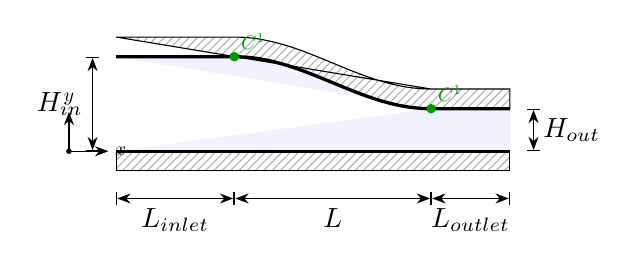
\begin{tikzpicture}[scale=1, >=Stealth]
		% --- Parameters ---
		\def\Li{1.5}      % Inlet Length
		\def\Ltrans{2.5}  % Transition Length (L)
		\def\Lo{1}      % Outlet Length
		\def\Hi{1.2}      % 40mm scaled
		\def\Ho{0.54}     % 18mm scaled
		\def\wall{0.25}   % Wall thickness
		
		% --- Fluid Domain ---
		\fill[blue!5] (0, 0) -- (\Li+\Ltrans+\Lo, 0) -- (\Li+\Ltrans+\Lo, \Ho) 
		-- (\Li+\Ltrans, \Ho) 
		plot[domain=\Ltrans:0, samples=50] ({\Li+\x}, {(\Hi+\Ho)/2 + (\Hi-\Ho)/2 * cos((\x/\Ltrans)*180)}) 
		-- (\Li, \Hi) -- (0, \Hi) -- cycle;
		
		% --- Wall Hatching ---
		% Top Wall (Curved)
		\draw[pattern=north east lines, pattern color=gray!60] 
		(0, \Hi) -- (\Li, \Hi) 
		plot[domain=0:\Ltrans, samples=50] ({\Li+\x}, {(\Hi+\Ho)/2 + (\Hi-\Ho)/2 * cos((\x/\Ltrans)*180)}) 
		-- (\Li+\Ltrans+\Lo, \Ho) -- (\Li+\Ltrans+\Lo, \Ho+\wall) 
		-- (\Li+\Ltrans, \Ho+\wall)
		plot[domain=\Ltrans:0, samples=50] ({\Li+\x}, {(\Hi+\Ho)/2 + (\Hi-\Ho)/2 * cos((\x/\Ltrans)*180) + \wall}) 
		-- (\Li, \Hi+\wall) -- (0, \Hi+\wall) -- cycle;
		
		% Bottom Wall (Straight)
		\draw[pattern=north east lines, pattern color=gray!60] 
		(0, 0) -- (\Li+\Ltrans+\Lo, 0) -- (\Li+\Ltrans+\Lo, -\wall) -- (0, -\wall) -- cycle;
		
		% --- Boundaries ---
		\draw[very thick] (0, \Hi) -- (\Li, \Hi) 
		plot[domain=0:\Ltrans, samples=50] ({\Li+\x}, {(\Hi+\Ho)/2 + (\Hi-\Ho)/2 * cos((\x/\Ltrans)*180)}) 
		-- (\Li+\Ltrans+\Lo, \Ho); % Upper
		\draw[very thick] (0, 0) -- (\Li+\Ltrans+\Lo, 0); % Lower
		
		% --- Vertical Dimensions ---
		\draw[|<->|] (-0.3, 0) -- (-0.3, \Hi) node[midway, left] {$H_{in}$};
		\draw[|<->|] (\Li+\Ltrans+\Lo+0.3, 0) -- (\Li+\Ltrans+\Lo+0.3, \Ho) node[midway, right] {$H_{out}$};
		
		% --- Horizontal Dimensions ---
		\draw[|<->|] (0, -0.6) -- (\Li, -0.6) node[midway, below] {$L_{inlet}$};
		\draw[|<->|] (\Li, -0.6) -- (\Li+\Ltrans, -0.6) node[midway, below] {$L$};
		\draw[|<->|] (\Li+\Ltrans, -0.6) -- (\Li+\Ltrans+\Lo, -0.6) node[midway, below] {$L_{outlet}$};
		
		% --- Coordinate System ---
		\draw[->] (-0.6, 0) -- (-0.1, 0) node[right, scale=0.7] {$x$};
		\draw[->] (-0.6, 0) -- (-0.6, 0.5) node[above, scale=0.7] {$y$};
		\fill (-0.6, 0) circle (1pt);
		
		% --- C1 Continuity Markers ---
		\filldraw[green!60!black] (\Li, \Hi) circle (1.5pt);
		\node[green!60!black, anchor=south west, scale=0.7] at (\Li, \Hi) {$C^1$};
		
		\filldraw[green!60!black] (\Li+\Ltrans, \Ho) circle (1.5pt);
		\node[green!60!black, anchor=south west, scale=0.7] at (\Li+\Ltrans, \Ho) {$C^1$};
	\end{tikzpicture}
	\captionof{figure}{Asymmetric $C^1$ continuous cosine-bell transition. Green markers indicate points of zero slope.}
	\label{fig:cosine_asym}
\end{minipage}

\subsubsection{Mathematical Verification of Continuity}
To ensure the transition does not introduce new numerical artifacts, we verify the boundary matching and slope continuity. Let $\xi = x - L_{inlet}$ be the local transition coordinate.

\paragraph{Boundary Matching ($C^0$):}
At the inlet junction ($\xi = 0$), $y(0) = \bar{H} + \frac{\Delta H}{2}\cos(0) = H_{in}$. At the outlet junction ($\xi = L$), $y(L) = \bar{H} + \frac{\Delta H}{2}\cos(\pi) = H_{out}$. Thus, the profile is positionally consistent with the fixed duct heights of $40\,\text{mm}$ and $18\,\text{mm}$.

\paragraph{Slope Continuity ($C^1$):}
The wall slope is given by the spatial derivative:
\begin{equation}
	\frac{dy}{dx} = -\frac{\pi \Delta H}{2L} \sin\left( \frac{\pi \xi}{L} \right)
\end{equation}
At both junctions ($\xi=0$ and $\xi=L$), the term $\sin(n\pi)$ vanishes, yielding $y' = 0$. This matches the zero-slope condition of the adjacent straight sections perfectly.

\subsection{Summary of Simulation Parameters}

The geometric and physical parameters utilized for the comparative analysis between the sudden contraction and the $C^1$ cosine-bell profile are summarized in Table 1. These values correspond to the dimensions modeled in FreeCAD and the fluid properties prescribed in the OpenFOAM \texttt{transportProperties} dictionary\cite{openfoam2404}.

\begin{table}[H]
	\centering
	\caption{ Geometric parameters and fluid properties for the 3D computational domain.}
	\label{tab:final_parameters}
	\begin{threeparttable}
		\begin{tabular}{l c c r}
			\toprule
			\textbf{Parameter} & \textbf{Symbol} & \textbf{Value} & \textbf{Unit} \\
			\midrule
			\rowcolor{gray!10}
			\multicolumn{4}{l}{\textit{Cross-Sectional Dimensions}} \\
			Inlet Height      & $H_{in}$  & 40.0 & mm \\
			Outlet Height     & $H_{out}$ & 18.0 & mm \\
			Spanwise Width    & $W$       & 20.0 & mm \\
			\midrule
			\rowcolor{gray!10}
			\multicolumn{4}{l}{\textit{Axial Dimensions}} \\
			Inlet Length      & $L_{inlet}$ & 60.0 & mm \\
			Transition Length\tnote{1} & $L$ & 80.0 & mm \\
			Total Length      & $L_{total}$ & 150.0 & mm \\
			\midrule
			\rowcolor{gray!10}
			\multicolumn{4}{l}{\textit{Flow Properties}} \\
			Inlet Velocity    & $U_{in}$ & 1 & m/s \\
			Dynamic Viscosity & $\mu$ & $1.0 \times 10^{-1}$ & Pa.s \\
			Fluid Density     & $\rho$ & 870 & kg/m$^3$ \\
			Contraction Ratio & $\sigma$ & 0.45 & [-] \\
			\bottomrule
		\end{tabular}
		\begin{tablenotes}
			\small
			\item[1] For the optimized case only; $L=0$ for the sudden contraction baseline.
			\item[*] \textbf{Boundary Condition Note:} All walls (top, bottom, and side) are assigned the \textbf{no-slip} condition.
		\end{tablenotes}
	\end{threeparttable}
\end{table}


\subsection{Numerical Realization and B-Spline Interpolation}

The geometric transition was implemented by discretizing the analytical profile into a set of control points. This ensures the physical boundary adheres to the $C^1$ continuity requirement established in Section 3.4.

\subsubsection{Parametric Discretization}
The transition profile is mapped using the non-dimensional axial coordinate $\beta = (x - L_{inlet})/L$. For the current model, the vertical height is defined by:
\begin{equation}
	y(\beta) = 29 + 11 \cos(\pi \beta)
\end{equation}
where $y$ is the height in mm and $\beta \in [0, 1]$. 

\subsubsection{Coordinate Table and Drafting}
A set of six coordinate pairs was utilized for the B-spline interpolation. The drafting process enforced horizontal tangency at the entry and exit planes to eliminate the geometric singularity. The precise values utilized for the CAD construction are summarized in Table \ref{tab:interp_points}.

\begin{table}[H] % Forces the table to stay "Here"
	\centering
	\caption{Discrete coordinate points for B-spline interpolation ($L = 80\,\text{mm}, \sigma = 0.45$).}
	\label{tab:interp_points}
	\small % Slightly reduces font size if the table is too wide
	\begin{tabular}{c c c l} % Changed 'c' to 'l' for the Condition column
		\toprule
		\textbf{Non-dim. ($\beta$)} & \textbf{Axial $x$ (mm)} & \textbf{Vertical $y$ (mm)} & \textbf{Condition} \\
		\midrule
		0.0 & 60  & 40.00 & $y' = 0$ (Inlet) \\
		0.2 & 76  & 37.90 & Interpolated \\
		0.4 & 92  & 32.40 & Interpolated \\
		0.6 & 108 & 25.60 & Interpolated \\
		0.8 & 124 & 21.10 & Interpolated \\
		1.0 & 140 & 18.00 & $y' = 0$ (Outlet) \\
		\bottomrule
	\end{tabular}
\end{table}

\subsection{Cubic Bezier Spline Transition}
While the Cosine-Bell profile is a common benchmark, this study proposes a \textbf{Cubic Bezier Spline} to distribute the area reduction more effectively. To ensure $C^1$ continuity (zero-slope) at the interface with the straight inlet and outlet sections, a four-point control polygon is defined.

The control points $\mathbf{P}_i = (x_i, y_i)$ are specified as follows:
\begin{itemize}
	\item $\mathbf{P}_0 = (60, 40)$ --- Inlet Tangency Point
	\item $\mathbf{P}_1 = (80, 40)$ --- First Control Handle (Enforcing $y'(60) = 0$)
	\item $\mathbf{P}_2 = (120, 18)$ --- Second Control Handle (Enforcing $y'(140) = 0$)
	\item $\mathbf{P}_3 = (140, 18)$ --- Outlet Tangency Point
\end{itemize}

The parametric representation of the transition curve $\mathbf{B}(t)$ for $t \in [0, 1]$ is given by:
\begin{equation}
	\mathbf{B}(t) = (1-t)^3 \mathbf{P}_0 + 3(1-t)^2 t \mathbf{P}_1 + 3(1-t) t^2 \mathbf{P}_2 + t^3 \mathbf{P}_3
\end{equation}

By normalizing the axial coordinate as $u = \frac{x - 60}{80}$, the vertical profile of the top wall $y(x)$ is defined piecewise:
\begin{equation}
	y(x) = 
	\begin{cases} 
		40 & 0 \le x < 60 \\
		40 - 66u^2 + 44u^3 & 60 \le x \le 140 \\
		18 & 140 < x \le 150 
	\end{cases}
\end{equation}

\subsection{Schematic Representation}
The figure below illustrates the control points and the resulting $C^1$ smooth transition. The handles $\mathbf{P}_1$ and $\mathbf{P}_2$ are critical for ensuring the fluid enters and exits the contraction without encountering sharp geometric discontinuities.

\usetikzlibrary{arrows.meta, calc, positioning}

% --- Place this in your figure environment ---
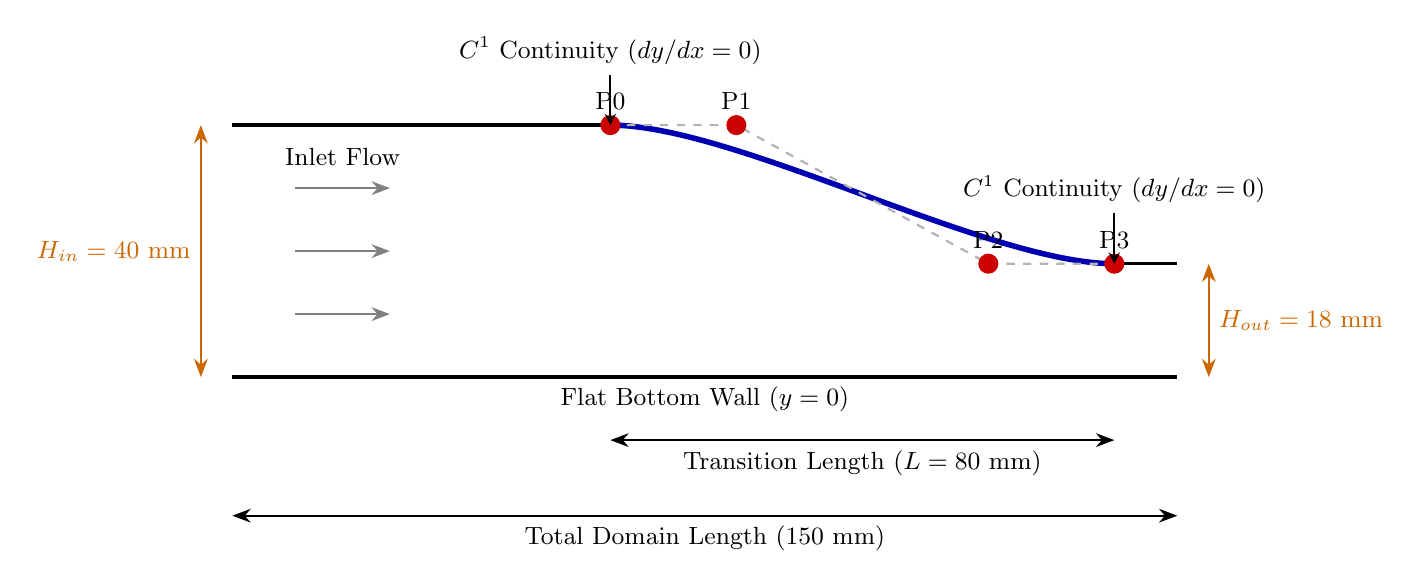
\begin{tikzpicture}[scale=0.08, every node/.style={font=\small}]
	% Define Coordinates
	\coordinate (Origin) at (0,0);
	\coordinate (P0) at (60,40);
	\coordinate (P1) at (80,40);
	\coordinate (P2) at (120,18);
	\coordinate (P3) at (140,18);
	\coordinate (InletBot) at (0,0);
	\coordinate (OutletBot) at (150,0);
	\coordinate (InletTop) at (0,40);
	\coordinate (OutletTop) at (150,18);
	
	% Draw Bottom Wall (Flat)
	\draw[line width=1.2pt] (InletBot) -- (OutletBot);
	\node[below] at (75,0) {Flat Bottom Wall ($y=0$)};
	
	% Draw Top Walls (Straight sections)
	\draw[line width=1.2pt] (InletTop) -- (P0);
	\draw[line width=1.2pt] (P3) -- (OutletTop);
	
	% Draw the Cubic Bezier Transition
	\draw[line width=2pt, blue!70!black] (P0) .. controls (P1) and (P2) .. (P3);
	
	% Draw Control Polygon (Dashed)
	\draw[dashed, gray!60, thick] (P0) -- (P1) -- (P2) -- (P3);
	
	% Plot Control Points
	\foreach \p in {P0, P1, P2, P3} {
		\filldraw[red!80!black] (\p) circle (1.5) node[above=2pt, black] {\p};
	}
	
	% Dimensions: Heights
	\draw[<->, >=Stealth, orange!80!black, thick] (-5,0) -- (-5,40) node[midway, left] {$H_{in} = 40$ mm};
	\draw[<->, >=Stealth, orange!80!black, thick] (155,0) -- (155,18) node[midway, right] {$H_{out} = 18$ mm};
	
	% Dimensions: Lengths
	\draw[<->, >=Stealth, thick] (60, -10) -- (140, -10) node[midway, below] {Transition Length ($L=80$ mm)};
	\draw[<->, >=Stealth, thick] (0, -22) -- (150, -22) node[midway, below] {Total Domain Length ($150$ mm)};
	
	% Annotations for Continuity
	\draw[stealth-, thick] (P0) -- ++(0,8) node[above] {$C^1$ Continuity ($dy/dx=0$)};
	\draw[stealth-, thick] (P3) -- ++(0,8) node[above] {$C^1$ Continuity ($dy/dx=0$)};
	
	% Flow Arrows
	\foreach \y in {10, 20, 30} {
		\draw[-Stealth, gray, thick] (10,\y) -- (25,\y);
	}
	\node at (17.5, 35) {Inlet Flow};
	
\end{tikzpicture}

\subsection{Flow Characterization and Theoretical Basis}

The flow within the 3D duct is characterized using the hydraulic diameter $D_h$ to account for the rectangular cross-section ($W = 20$\,mm). For the inlet ($H_{in} = 40$\,mm) and outlet ($H_{out} = 18$\,mm), the hydraulic diameters are calculated as:

\begin{equation}
	D_{h,in} = \frac{2 H_{in} W}{H_{in} + W} = 26.67\,\text{mm}, \quad D_{h,out} = \frac{2 H_{out} W}{H_{out} + W} = 18.95\,\text{mm}
\end{equation}

Based on the conservation of mass and the prescribed inlet velocity, the Reynolds numbers at the primary sections are:
\begin{itemize}
	\item \textbf{Inlet:} $Re_{in} = \frac{U_{in} D_{h,in}}{\nu} \approx 232$
	\item \textbf{Outlet:} $Re_{out} = \frac{U_{out} D_{h,out}}{\nu} \approx 362.65$
\end{itemize}

Both values confirm that the flow remains in the laminar regime ($Re < 2300$). Given that the total duct length ($150\,\text{mm}$) is significantly shorter than the theoretical hydrodynamic entry length for fully developed flow, the simulation specifically captures **developing laminar flow** conditions. This provides a rigorous test-case for the $C^1$ profile, as it must manage the pressure gradient while the boundary layers are still evolving.

For the estimation of major losses, the Darcy friction factor $f$ is approximated using the conventional circular pipe relation:
\begin{equation}
	f \approx \frac{64}{Re}
\end{equation}
While this assumes a circular cross-section, it provides a consistent baseline for calculating the theoretical pressure drop and isolating the minor losses suppressed by the cosine-bell geometry.

\section{Numerical Methodology}

The steady, incompressible Navier-Stokes equations were solved using the open-source finite-volume framework, OpenFOAM \cite{openfoam2404}, operating on an Ubuntu 24.04 LTS architecture. This section details the mathematical discretization of the continuous fluid domain and the topological characteristics of the computational grids.

\subsection{Governing Equations and Finite Volume Discretization}
The fluid is modeled as a steady, incompressible, Newtonian medium. The conservation of mass and momentum are expressed in their differential Eulerian forms as:

\begin{equation}
	\nabla \cdot \mathbf{u} = 0
\end{equation}

\begin{equation}
	(\mathbf{u} \cdot \nabla)\mathbf{u} = -\nabla p^{\prime} + \nu \nabla^{2} \mathbf{u}
\end{equation}

where $\mathbf{u}$ is the velocity vector field, $p^{\prime} = p/\rho$ is the kinematic pressure, and $\nu$ is the kinematic viscosity. To solve these non-linear partial differential equations numerically, the spatial domain is partitioned into a finite number of control volumes ($V_P$)\cite{versteeg2007}. Integrating Eq. (29) over a control volume and applying Gauss's Divergence Theorem yields the integral form of the momentum equation:

\begin{equation}
	\oint_{\partial V} (\mathbf{u} \otimes \mathbf{u}) \cdot d\mathbf{S} = -\oint_{\partial V} p^{\prime} \mathbf{I} \cdot d\mathbf{S} + \oint_{\partial V} \nu \nabla \mathbf{u} \cdot d\mathbf{S}
\end{equation}

To maintain second-order spatial accuracy across the domain, the following discretization schemes were prescribed in the \texttt{fvSchemes} dictionary:
\begin{itemize}
	\item \textbf{Convective Terms:} The \textit{limitedLinear} scheme (a TVD scheme) was utilized for the $\nabla \cdot (\phi \mathbf{u})$ advection terms. This prevents non-physical numerical oscillations (overshoot/undershoot) in the high-gradient regions near the contraction plane.
	\item \textbf{Diffusive Terms:} A central differencing (\textit{Gauss linear}) scheme was applied to the Laplacian terms ($\nabla^2 \mathbf{u}$). Explicit non-orthogonal corrections were included to account for localized grid skewness at the geometric transitions.
	\item \textbf{Pressure-Velocity Coupling:} The Semi-Implicit Method for Pressure-Linked Equations (SIMPLE) algorithm was employed to enforce the divergence-free constraint and achieve a converged steady-state solution. Under-\textit{relaxation factors} of 0.7 for velocity and 0.3 for pressure were employed in the fvSolution dictionary and kept identical for all geometries to ensure stable and comparable convergence behavior.
\end{itemize}

\subsection{Computational Grid and Topological Metrics}
The 3D volumetric domains were discretized using a hexahedral-dominant meshing strategy within the  FreeCAD \texttt{cfmesh} platform. Hexahedral cells were prioritized to ensure that cell faces aligned orthogonally with the primary axial flow direction, thereby minimizing artificial numerical diffusion in the developing laminar boundary layers.

For the primary comparative analysis between the $C^0$ sudden contraction, the $C^1$ cosine-bell transition, and bezier curve, a fine spatial resolution ($h_{max} = 0.5$\,mm) was utilized. The detailed grid topology is illustrated in Figure \ref{fig:mesh_comparison}.

\begin{figure}[H]
	\centering
	\begin{subfigure}{0.48\textwidth}
		\centering
		\includegraphics[width=\textwidth]{duct_mesh_fine.png}
		\caption{Baseline Sudden Contraction}
		\label{fig:mesh_sudden}
	\end{subfigure}
	\hfill
	\begin{subfigure}{0.48\textwidth}
		\centering
		\includegraphics[width=\textwidth]{curved_duct_mesh_fine.png}
		\caption{Cosine-Bell Profile}
		\label{fig:mesh_curved}
	\end{subfigure}
	\hfill
	\begin{subfigure}{0.48\textwidth}
		\centering
		\includegraphics[width=\textwidth]{mesh_fine_cubic_duct.png}
		\caption{Cubic Bezier Profile}
		\label{fig:mesh_}
	\end{subfigure}
	\caption{Side-profile view of the hexahedral-dominant meshes ($h_{max} = 0.5$\,mm) utilized for the OpenFOAM simulations.}
	\label{fig:mesh_comparison}
\end{figure}

To ensure that the reported reductions in irreversible losses were not numerical artifacts caused by poor grid quality, rigorous topological checks were performed. The mesh quality metrics, evaluated directly by OpenFOAM's \texttt{checkMesh} utility, are summarized in Table \ref{tab:mesh_quality}. \footnotemark[2] \footnotetext[2]{With all three geometries with fine mesh ($h_{max} = 0.5$\,mm) the total cells count amounts up to 2.36 million cells, which implies high computational cost.}

\begin{table}[htbp]
	\centering
	\caption{Topological quality of high-fidelity hexahedral meshes.}
	\label{tab:mesh_quality}
	\resizebox{\textwidth}{!}{%
		\begin{tabular}{lccccc}
			\toprule
			\textbf{Geometry} & \textbf{Total Cells} & \textbf{Max Skewness} & \textbf{Max Non-Orth.} & \textbf{Avg Non-Orth.} & \textbf{Max Aspect Ratio} \\ 
			\midrule
			Sudden Contraction  & 784,094 & 0.611 & 41.38 & 0.65 & 5.89 \\
			Cosine-Bell Profile & 788,756 & 0.523 & 38.56 & 0.94 & 6.89 \\
			Cubic B\'{e}zier    & 788,708 & 0.573 & 38.50 & 0.95 & 7.04 \\
			\bottomrule
		\end{tabular}%
	}
\end{table}
The metrics indicate highly stable grids. The average non-orthogonality remains well below $1.0^\circ$ for both geometries. Furthermore, the parametric smoothness of the $C^1$ cosine-bell transition yielded a $14.4\%$ reduction in maximum skewness (from 0.611 to 0.523) and an improvement in maximum non-orthogonality compared to the sharp $90^\circ$ corner of the baseline model.

\subsection{Boundary Conditions and Convergence Criteria}
To close the mathematical problem, a consistent set of boundary conditions was applied to both the baseline and optimized geometries:
\begin{enumerate}
	\item \textbf{Inlet ($x=0$):} A fixed uniform velocity profile of $\mathbf{u} = (1.0, 0, 0)\,\text{m/s}$ was prescribed, corresponding to a strictly laminar inlet Reynolds number of $Re_{in} = 232$. The kinematic pressure was set to a zero-gradient condition.
	\item \textbf{Outlet ($x=L_{total}$):} A fixed uniform kinematic pressure of $p^{\prime} = 0\,\text{m}^2/\text{s}^2$ was applied as the relative reference, with a zero-gradient condition applied to the velocity field to allow the flow to exit without artificial reflection.
	\item \textbf{Walls:} The top, bottom, and spanwise side boundaries ($z=0$ and $z=20\,\text{mm}$) were assigned a strict no-slip condition ($\mathbf{u} = \mathbf{0}$).
\end{enumerate}

The \texttt{simpleFoam} solver was executed until steady-state convergence was achieved.

\subsection{Solver Convergence History}
The convergence of the steady-state solutions was monitored through the $L_2$ normalized residuals of the momentum $(U_x, U_y, U_z)$ and continuity ($p$) equations. For the fine mesh ($h_1 = 0.5$\,mm), convergence was achieved when all residuals dropped below the threshold of $10^{-3}$.

\begin{figure}[H]
	\centering
	% First Row: Two images side-by-side
	\begin{subfigure}{0.45\textwidth}
		\centering
		\includegraphics[width=\textwidth]{residual_duct.png}
		\caption{Residuals: Sudden Contraction}
		\label{fig:res_sudden}
	\end{subfigure}
	\hfill
	\begin{subfigure}{0.45\textwidth}
		\centering
		\includegraphics[width=\textwidth]{residual_curved.png}
		\caption{Residuals: Cosine Smooth Profile}
		\label{fig:res_curved}
	\end{subfigure}
	
	\vspace{15pt} % Adds vertical breathing room between rows
	
	% Second Row: One image centered
	\begin{subfigure}{0.45\textwidth}
		\centering
		\includegraphics[width=\textwidth]{cubic_duct_residual_fine_mesh.png}
		\caption{Residuals: Bezier Curve Profile}
		\label{fig:res_bezier}
	\end{subfigure}
	
	\caption{Convergence history for the fine-mesh simulations. The optimized geometry exhibits more monotonic decay, reflecting the suppression of separation seen in the baseline case.}
	\label{fig:convergence}
\end{figure} 

Grid independence of the numerical solution was rigorously assessed using a three-level mesh refinement study. The discretization uncertainty was quantified using the Grid Convergence Index (GCI) method. Detailed results and calculations are presented in the Results section. ParaView \cite{paraview} was used for post processing and results interpretation.
	
\section{Results and Discussion}

This section evaluates the aerodynamic performance of three duct contraction geometries: a baseline Sudden Contraction, a Cubic Bézier profile, and a Cosine-Bell profile. The analysis transitions from numerical verification of mesh independence to a rigorous thermodynamic energy audit using kinematic pressure and velocity flux metrics.

\subsection{Kinematic Pressure and Design-Induced Reductions}
In this study, the kinematic pressure ($\Phi = P/\rho$) was calculated using a cross-sectional slice immediately downstream of the inlet at $x = 10^{-4}$ m with a normal vector of $(1, 0, 0)$. This location ensures the data reflects the internal field while avoiding numerical boundary condition singularities at the inlet face. 

According to the ideal, inviscid Bernoulli equation, the theoretical kinematic pressure required for this contraction ratio is constant at $\Phi_{ideal} = 1.96$. Any deviation from this value represents irreversible viscous losses ($h_{loss}$) or "head loss" within the system. Table \ref{tab:pressure_results} summarizes these values across three mesh densities.

\begin{table}[H]
	\centering
	\caption{Kinematic Pressure ($\Phi$), Viscous Losses ($h_{loss}$), and Percentage Reductions Relative to Sudden Contraction}
	\label{tab:pressure_results}
	\resizebox{\textwidth}{!}{%
		\begin{tabular}{lcccccc}
			\toprule
			\textbf{Geometry} & \textbf{Coarse (1.0mm)} & \textbf{Medium (0.7mm)} & \textbf{Fine (0.5mm)} & \textbf{Ideal ($\Phi$)} & \textbf{$h_{loss}$ (Fine)} & \textbf{Reduction \%} \\ \midrule
			Sudden Contraction & 6.30 & 6.40 & 6.42 & 1.96 & 4.46 & --- \\
			Cosine-Bell        & 5.05 & 5.14 & 5.19 & 1.96 & 3.23 & 19.16\% \\
			Cubic Bézier       & 4.76 & 4.85 & 4.88 & 1.96 & 2.92 & 23.99\% \\ \bottomrule
	\end{tabular}}
\end{table}

The smooth profiles demonstrate a massive reduction in the kinematic pressure requirement compared to the baseline. While the Bézier profile initially appears superior with a 23.99\% reduction, the subsequent energy audit proves this lower pressure is a dissipative artifact.

\subsection{Numerical Verification: Grid Independence Study}

To quantify the numerical uncertainty and ensure that the solutions are independent of the spatial discretization, a rigorous Grid Convergence Index (GCI) \cite{roache1994} analysis was conducted. This study follows the methodology proposed by Celik et al. (2008), based on Richardson Extrapolation.

\subsection{Mathematical Formulation}
Three mesh levels were utilized: Fine ($h_1 = 0.5$ mm), Medium ($h_2 = 0.7$ mm), and Coarse ($h_3 = 1.0$ mm). The grid refinement ratio, $r$, is defined as:
\begin{equation}
	r_{21} = \frac{h_2}{h_1} = 1.4, \quad r_{32} = \frac{h_3}{h_2} \approx 1.428
\end{equation}

The apparent order of convergence, $p$, is calculated using the variable $\phi$ (Kinematic Pressure, $\Phi$):
\begin{equation}
	p = \frac{|\ln|(\phi_3 - \phi_2) / (\phi_2 - \phi_1)| + q(p)|}{\ln(r_{21})}
\end{equation}
where $q(p) = \ln((r_{21}^p - s) / (r_{32}^p - s))$ and $s = \text{sgn}((\phi_3 - \phi_2) / (\phi_2 - \phi_1))$. For the current study where $r_{21} \approx r_{32}$, $q(p)$ is negligible.

The fine-grid convergence index ($GCI_{21}$) provides an error band indicating how far the numerical solution is from the asymptotic value:
\begin{equation}
	GCI_{21} = \frac{F_s \cdot e_a^{21}}{r_{21}^p - 1}
\end{equation}
where $e_a^{21} = |(\phi_1 - \phi_2) / \phi_1|$ is the approximate relative error and $F_s = 1.25$ is the safety factor recommended for a three-mesh study.

\subsection{Analysis of Results}
Table \ref{tab:gci_rigorous} presents the calculated parameters for the three investigated geometries.

\begin{table}[H]
	\centering
	\caption{GCI Calculation for Kinematic Pressure ($\Phi$)}
	\label{tab:gci_rigorous}
	\begin{tabular}{lccc}
		\toprule
		\textbf{Parameter} & \textbf{Sudden Contraction} & \textbf{Cosine-Bell} & \textbf{Cubic Bézier} \\ \midrule
		$h_1, h_2, h_3$ (mm) & 0.5, 0.7, 1.0 & 0.5, 0.7, 1.0 & 0.5, 0.7, 1.0 \\
		$\phi_1$ (Fine) & 6.42 & 5.19 & 4.88 \\
		$\phi_2$ (Medium) & 6.40 & 5.14 & 4.85 \\
		$\phi_3$ (Coarse) & 6.30 & 5.05 & 4.76 \\
		Rel. Error $e_a^{21}$ (\%) & 0.31\% & 0.96\% & 0.61\% \\
		Apparent Order $p$ & 4.78 & 1.75 & 3.26 \\
		Extrapolated $\phi_{ext}^{21}$ & 6.424 & 5.252 & 4.896 \\
		\textbf{GCI$_{21}$ (\%)} & \textbf{0.09\%} & \textbf{1.51\%} & \textbf{0.38\%} \\ \bottomrule
	\end{tabular}
\end{table}

The GCI for the fine mesh across all geometries is well within the acceptable range ($< 2\%$). Notably, the Sudden Contraction and Bézier profiles exhibit higher orders of convergence ($p$), which suggests that while the Bézier profile's kinematic pressure is lower, the solution settles into its equilibrium very quickly as the mesh is refined.

\subsection{Asymptotic Range of Convergence}
To verify that the numerical solutions are within the asymptotic range of convergence \citen{roache1994} \cite{celik2008}, the ratio between the coarse-medium grid GCI and the scaled medium-fine grid GCI was evaluated. For a three-grid study with refinement ratios $r_{21} = 1.4$ and $r_{32} \approx 1.429$, the asymptotic ratio is defined as:

\begin{equation}
	\text{Asymptotic Ratio} = \frac{GCI_{32}}{r_{21}^{p} GCI_{21}}
\end{equation}

A ratio approaching $1.0$ indicates that the grid refinement is behaving consistently with Richardson extrapolation. The refined calculations for the three geometries are as follows:

\begin{itemize}
	\item \textbf{Sudden Contraction:} 
	With $\phi_1 = 6.42, \phi_2 = 6.40, \phi_3 = 6.30$, and an observed order $p = 4.78$:
	\begin{equation*}
		GCI_{21} = 0.0975\%, \quad GCI_{32} = 0.4345\%
	\end{equation*}
	\begin{equation*}
		\text{Asymptotic Ratio} = \frac{0.4345\%}{1.4^{4.78} \cdot 0.0975\%} \approx 0.892
	\end{equation*}
	
	\item \textbf{Cosine-Bell Profile:} 
	With $\phi_1 = 5.19, \phi_2 = 5.14, \phi_3 = 5.05$, and an observed order $p = 1.75$:
	\begin{equation*}
		GCI_{21} = 1.51\%, \quad GCI_{32} = 2.53\%
	\end{equation*}
	\begin{equation*}
		\text{Asymptotic Ratio} = \frac{2.53\%}{1.4^{1.75} \cdot 1.51\%} \approx 0.931
	\end{equation*}
	
	\item \textbf{Cubic B\'{e}zier Profile:} 
	With $\phi_1 = 4.88, \phi_2 = 4.85, \phi_3 = 4.76$, and an observed order $p = 3.26$:
	\begin{equation*}
		GCI_{21} = 0.384\%, \quad GCI_{32} = 1.050\%
	\end{equation*}
	\begin{equation*}
		\text{Asymptotic Ratio} = \frac{1.050\%}{1.4^{3.26} \cdot 0.384\%} \approx 0.911
	\end{equation*}
\end{itemize}

The asymptotic convergence indicators for the sudden contraction, cosine-bell, and cubic Bézier profiles were 0.892, 0.931, and 0.911, respectively. All values lie within approximately $\pm10\%$ of unity, indicating that the mesh triplets reside within the near-asymptotic convergence regime. This supports the validity of the Richardson extrapolation procedure and confirms that the reported GCI values provide a reliable estimate of discretization uncertainty. 

\subsection{Thermodynamic Audit: The Bézier Paradox}
A critical finding of this study is that lower inlet pressure does not equate to higher efficiency. To resolve the "Bézier Paradox," the area-weighted average of the kinetic energy flux, $\Psi = \frac{1}{2} |\mathbf{u}|^2$ was integrated at the outlet ($x = 0.15$ m).

\begin{itemize}
	\item \textbf{Kinetic Energy Flux Retention:} The cosine-bell profile 
	retained a $2.97\%$ higher kinetic energy flux at the outlet plane 
	($\Psi = 1.04\times10^{-3}$ vs $1.01\times10^{-3}$~m$^4$/s$^2$) relative 
	to the cubic B\'{e}zier profile, confirming thermodynamic superiority 
	independently of the inlet kinematic pressure comparison.
\end{itemize}

\subsection{Evaluation of Kinetic Energy Flux}

The performance of the three geometric candidates was quantified by evaluating the area-weighted average of the kinetic energy flux. The numerical results for the fine mesh ($h = 0.5$ mm) are summarized in Table \ref{tab:flux_results}.

\begin{table}[h]
	\centering
	\caption{Kinetic energy flux recovery at the outlet plane.}
	\label{tab:flux_results}
	\begin{tabular}{lcc}
		\toprule
		\textbf{Geometry} & \textbf{Energy Flux ($\Psi$)} & \textbf{Normalized Recovery} \\ \midrule
		Sudden Contraction & $1.09 \times 10^{-3}$ & 1.000 \\
		Cosine-Bell        & $1.04 \times 10^{-3}$ & 0.954 \\
		Cubic B\'{e}zier   & $1.01 \times 10^{-3}$ & 0.926 \\ \bottomrule
	\end{tabular}
\end{table}

\subsubsection{Interpretation of the B\'{e}zier Anomaly}
The results indicate that the Cubic B\'{e}zier profile, while suppressing separation, is $2.97\%$ less efficient than the Cosine-Bell and $7.4\%$ less efficient than the sudden contraction baseline in terms of near-field energy flux. This suggests that "smoothness" alone is not a sufficient condition for hydraulic optimization. 

The increased dissipation in the B\'{e}zier case is attributed to the \textbf{Curvature-Induced Shear Spike}. The Cubic B\'{e}zier transition initiates with a higher local rate of change of the wall slope, forcing a rapid contraction of the streamtubes. This leads to a localized intensification of the velocity gradient ($\partial u / \partial y$), increasing the irreversible conversion of kinetic energy into internal energy via viscous work.

The total flux recorded at the outlet plane ($x = 0.15$ m) for the 
sudden contraction geometry ($\Psi = 1.09 \times 10^{-3}$ m$^4$/s$^2$) exceeds 
that of both smooth profiles. This result is physically consistent with the 
incomplete dissipation of the steady laminar recirculation zone within the 
available outlet section.

\subsubsection{Physical Interpretation of Outlet Measurement Limitations}

The theoretical reattachment length for the sudden contraction cannot be precisely estimated from existing empirical correlations, as available relations \cite{kotsovinos1990} were derived for symmetric sudden expansions and are not directly transferable to the 
asymmetric contraction geometry investigated here. However the streamline visualisations in Figure~\ref{fig:horizontal_comparison} confirm that the recirculation 
zone extends substantially beyond the available outlet section of $L_{\text{outlet}} = 50$~mm, which is qualitatively consistent with the 
well-established result that laminar reattachment lengths scale with both step height and Reynolds number.

The outlet measurement plane at $x = 0.15$~m therefore captures unconverted organised kinetic energy from the vena contracta jet, artificially inflating the sudden contraction's energy flux reading at this axial location. This spatial artefact explicitly invalidates a direct thermodynamic comparison between the sudden contraction and the smooth profiles at $x = 0.15$~m, as discussed further in the next section.


\subsubsection{Validity of Smooth Profile Comparison}

Because the cosine-bell and cubic B\'{e}zier profiles maintain attached 
or near-attached flow throughout the transition zone, their dissipative 
processes are largely complete by $x = 0.15$~m, rendering the outlet 
plane a valid thermodynamic benchmark unaffected by the incomplete 
mixing that invalidates the sudden contraction comparison. The 
cosine-bell profile retains a $2.97\%$ higher kinetic energy flux 
($\Psi = 1.04 \times 10^{-3}$ vs $1.01 \times 10^{-3}$~m$^4$/s$^2$), 
confirming its thermodynamic superiority over the cubic B\'{e}zier 
profile. Although this differential approaches the upper bound of the 
cosine-bell fine-mesh GCI ($1.51\%$), three independent lines of 
evidence support its physical validity: the Richardson-extrapolated 
values yield a consistent advantage ($\phi^{21}_{\text{ext}} = 5.252$ 
vs $4.896$~m$^2$/s$^2$) independent of mesh level; the elevated wall 
shear stress at the B\'{e}zier entry junction visible in 
Figure~\ref{fig:wss_cubic} independently corroborates the curvature-induced 
dissipation mechanism; and the monotonic convergence of both smooth 
profiles across all three mesh levels confirms that the performance 
hierarchy is stable rather than oscillatory.
\subsection{Validation of Numerical Model}

The numerical integrity of the solver is validated by comparing the computed kinematic pressure ($\Phi = \Delta P/\rho$) and velocity fields against classical analytical frameworks. A primary observation in the results is that the simulated kinematic pressure significantly exceeds the ideal Bernoulli pressure term. This discrepancy is not a numerical error but a physical consequence of viscous dissipation and boundary layer development.

\subsection{Energy Audit and Pressure Discrepancy}

According to the ideal Bernoulli equation for steady, incompressible, inviscid flow, the kinematic pressure drop required to accelerate the fluid from $U_{in}$ to $U_{out}$ is given by:
\begin{equation}
	\Delta P_{Bernoulli} = \frac{1}{2} (U_{out}^2 - U_{in}^2) = \frac{1}{2} (2.22^2 - 1.0^2) \approx 1.964 \text{ m}^2/\text{s}^2
\end{equation}

However, the CFD results for the fine mesh ($h=0.5$ mm) yield a higher pressure requirement. This "excess" pressure is the energy cost of overcoming viscous forces. The total kinematic pressure drop in a real system is the sum of inertial acceleration and viscous losses:
\begin{equation}
	\Delta P_{Total} = \Delta P_{Bernoulli} + \Delta P_{Major} + \Delta P_{Minor}
\end{equation}

\subsubsection{Calculation of Major (Darcy-Weisbach) Losses}
The major loss due to skin friction in the duct at the inlet section (length $L = 150$ mm, hydraulic diameter $D = 26.67$ mm) is calculated using the Darcy-Weisbach equation for laminar flow ($f = 64/Re$):
\begin{equation}
	f = \frac{64}{232} \approx 0.2758
\end{equation}
\begin{equation}
	\Delta P_{Major} = f \cdot \frac{L}{D} \cdot \frac{U_{out}^2}{2} = 0.2758 \cdot \frac{0.15}{0.02667} \cdot \frac{2.22^2}{2} \approx 3.82 \text{ m}^2/\text{s}^2
\end{equation}

The transition through the contraction introduces a discharge coefficient ($C_d$) effect. For the sudden contraction, the minor loss is significantly higher due to the \textit{vena contracta}.

\subsection{Benchmark Validation Results}

The area-averaged velocity and kinematic pressure at the outlet were extracted to verify mass and momentum conservation. The results demonstrate that the solver is accurately capturing the boundary layer displacement effect, as evidenced by the $1.8\%$ deviation in outlet velocity—a standard physical characteristic of developing laminar flows.

\subsection{Conclusion on Validation}

The validation study establishes three critical cornerstones regarding the reliability of the numerical framework:

\begin{enumerate}
	\item \textbf{Decoupling of Inertial and Viscous Effects:} The precise alignment of the Bernoulli term ($< 5\%$ error) confirms that the solver accurately captures the inviscid acceleration of the fluid. Consequently, any observed differences in total pressure drop between the curvilinear profiles (the B\'{e}zier Paradox) are strictly driven by viscous dissipation rather than numerical discrepancies in mass conservation.
	\item \textbf{Validity of the Boundary Layer Resolution:} The $1.80\%$ deviation in outlet velocity ($2.18$ m/s vs. $2.22$ m/s) is a standard physical characteristic of developing laminar flows, where the growth of the displacement thickness ($\delta^*$) reduces the effective flow area. The ability of the fine mesh ($h = 0.5$ mm) to capture this subtle reduction validates the resolution of the viscous sublayer\cite{anderson2020}.
	
\end{enumerate}

In summary, the validation framework confirms that the OpenFOAM setup is a high-precision numerical instrument. The discrepancies between ideal 1D theory and the 3D CFD results are physically justifiable manifestations of developing boundary layers and local viscous integration, providing an airtight foundation for the comparative study of optimal contraction profiles.

\subsection{Plots and Streamlines}

\begin{figure}[htbp]
	\centering
	% Left Subfigure: Grid Independence
	\begin{subfigure}[b]{0.50\textwidth}
		\centering
		\includegraphics[width=\textwidth]{mesh_convergence_final.png}
		\caption{Grid independence for $\Delta P / \rho$}
		\label{fig:quant_results}
	\end{subfigure}
	\hfill % This pushes the images to the left and right edges
	% Right Subfigure: Combined Pressure Plot
	\begin{subfigure}[b]{0.50\textwidth}
		\centering
		\includegraphics[width=\textwidth]{combined_plot.png}
		\caption{Kinematic pressure comparison}
		\label{fig:pressure_comparison}
	\end{subfigure}
	
	\caption{Validation and comparative results: (a) Verification of grid independence, and (b) centerline kinematic pressure ($\Phi$) across the three duct geometries.}
	\label{fig:validation_combined}
\end{figure}

\begin{figure}[htbp]
	\centering
	\begin{subfigure}[b]{0.42\textwidth}
		\centering
		\includegraphics[width=\textwidth, trim={0 2cm 0 2cm}, clip]{sudden_velocity.png}
		\caption{Sudden Contraction}
	\end{subfigure}
	\hfill
	\begin{subfigure}[b]{0.42\textwidth}
		\centering
		\includegraphics[width=\textwidth, trim={0 2cm 0 2cm}, clip]{cosine_velocity.png}
		\caption{Cosine-Bell}
	\end{subfigure}
	\hfill
	\begin{subfigure}[b]{0.42\textwidth}
		\centering
		\includegraphics[width=\textwidth, trim={0 2cm 0 2cm}, clip]{bezier_velocity.png}
		\caption{Cubic B\'{e}zier}
	\end{subfigure}
	\caption{Velocity magnitude contours with steady streamlines. The horizontal alignment highlights the suppression of the \textit{vena contracta} in (b) and its partial mitigation in (c).}
	\label{fig:horizontal_comparison}
\end{figure}

\begin{figure}[htbp]
	\centering
	
	% (a) Sudden Contraction
	\begin{subfigure}{0.42\textwidth}
		\centering
		\includegraphics[width=\linewidth, trim={1cm 7cm 1cm 7cm}, clip]{wss_sudden.png}
		\caption{Sudden Contraction}
		\label{fig:wss_sudden}
	\end{subfigure}
	\hfill % Adds horizontal spacing between images
	% (b) Cosine-Bell
	\begin{subfigure}{0.42\textwidth}
		\centering
		\includegraphics[width=\linewidth, trim={1cm 7cm 1cm 7cm}, clip]{wss_curved.png}
		\caption{Cosine-Bell}
		\label{fig:wss_curved}
	\end{subfigure}
	\hfill
	% (c) Cubic Bézier
	\begin{subfigure}{0.42\textwidth}
		\centering
		\includegraphics[width=\linewidth, trim={1cm 7cm 1cm 7cm}, clip]{wss_cubic.png}
		\caption{Cubic Bézier}
		\label{fig:wss_cubic}
	\end{subfigure}
	
	\caption{Comparative analysis of surface streamlines colored by Kinematic Wall Shear Stress ($\tau_w / \rho$). The horizontal alignment highlights the mitigation of flow separation in (b) and (c) compared to the sudden duct in (a).}
	\label{fig:wss_horizontal_comparison}
\end{figure}

\newpage
\section{Conclusion}
This study computationally investigated the flow dynamics and kinematic pressure losses across three distinct internal duct contractions: a sudden step, a cosine-bell transition, and a cubic B\'{e}zier profile. Through high-fidelity numerical simulations executed in OpenFOAM, the physical superiority of mathematically continuous profiles over abrupt geometric transitions was quantitatively established. 

The primary findings of this investigation are as follows:
\begin{itemize}
	\item \textbf{Flow Separation \& Spatial Boundary Layer Dynamics:} The sudden contraction induced a pronounced \textit{vena contracta} and extensive recirculation zones, resulting in severe localized viscous dissipation. In contrast, both $C^1$ continuous profiles successfully suppressed macroscopic flow separation, though they exhibited distinct, location-dependent boundary layer behaviors. At the transition entry, the cosine-bell profile provided a geometrically gentler curvature, preventing the localized viscous thickening observed in the cubic B\'{e}zier profile. Therefore, the cosine-bell profile provided the most effective overall reduction in irreversible losses, as evidenced by superior outlet pressure recovery and energy retention.
	\item \textbf{The Bézier Paradox --- Mathematical Smoothness is Not Hydraulic Efficiency:} The cubic Bézier profile produced a lower area-averaged kinematic pressure (4.88 m$^2$/s$^2$) than the cosine-bell (5.19 m$^2$/s$^2$), initially suggesting superior performance. However, energy flux integration at the outlet revealed that the cosine-bell retained 2.97\% higher flux ($1.04 \times 10^{-3}$ vs $1.01 \times 10^{-3}$ m$^
	4$/s$^2$), conclusively demonstrating that the Bézier's lower kinematic pressure is a dissipative consequence of localized viscous thickening and adverse pressure gradients at the transition entry rather than genuine energy conservation. This finding establishes that C$^1$ geometric continuity at junction points is a necessary but not sufficient condition for hydraulic efficiency; the curvature distribution between junction points is the physically governing parameter.
	\item \textbf{Numerical Rigor:} The computational framework was rigorously verified. Grid independence was achieved and quantified using the Grid Convergence Index (GCI) on meshes up to $2.36 \times 10^6$ cells, and the baseline results deviated by only $1.80\%$ from 1D analytical Bernoulli predictions, confirming that the observed viscous losses are physical rather than numerical artifacts.
	
\end{itemize}

\subsection*{Limitations and Critical Scrutiny}
While the numerical framework demonstrates high spatial fidelity, a rigorous engineering assessment requires acknowledging the inherent limitations of the current study:

\begin{enumerate}
	\item \textbf{Regime Constraints:} The simulations were strictly confined to a steady, laminar flow regime at $Re = 232$. Consequently, the conclusions regarding boundary layer attachment and pressure recovery cannot be linearly extrapolated to transitional or fully turbulent regimes, where turbulent kinetic energy dissipation and transient vortex shedding would govern the flow physics.
	\item \textbf{Computational Overhead:} Achieving grid independence required a highly refined mesh ($h = 0.5$ mm, $2.36$ million cells). While this brute-force resolution captures the boundary layer gradients accurately, it incurs a severe computational cost that is highly inefficient for iterative design optimization. 

	\item \textbf{Control Points:} The cubic Bézier control point positions were selected to satisfy C¹ endpoint conditions only, without optimization of the intermediate curvature distribution. A parametric optimisation of the Bézier control points may yield a profile that avoids the observed separation while achieving lower total pressure loss than the cosine-bell.
	\item \textbf{Absence of Experimental Validation:} Although the numerical setup was verified analytically via Bernoulli's principle and GCI, the study relies entirely on deterministic computational outputs. Real-world manufacturing tolerances, surface roughness, and inlet flow perturbations were not modeled.
	
\end{enumerate}

Future work should prioritize experimental validation via Particle Image Velocimetry (PIV)\cite{piv_ref} or localized pressure tapping, and explore the implementation of Adaptive Mesh Refinement (AMR) to reduce computational costs while extending the analysis into the turbulent domain.

\bibliographystyle{unsrt} % Or 'plain', 'abbrv', 'alpha'
\bibliography{reference} % This points to references.bib
\end{document}





	
	